\section{图}
正文内容。插图尽可能不用彩色图。小图宽度小于7.5 cm,大图宽度为12~15cm 。图必须有中英文图序、图题。函数图只在靠近坐标线处残留一小段标值短线,其余部分省略。加注坐标所代表的量及单位(如t/s)。标值排印在坐标外侧,紧靠标值短线的地方;标值的有效数字为3位。图中量的意义要在正文中加以解释。若有图注,靠近放在图下部,图序、图题的上方。

\begin{figure}[H]
	\centering
	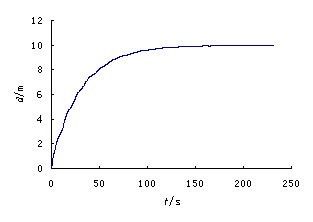
\includegraphics[width=3in]{sections/figs/template.png}
	\caption{\label{fig1111} \xiaowuhao \hei 图题}
\end{figure}

\section{数学符号和数学式的编排规范}
正文内容。变量、变动附标及函数用斜体字母表示。点、线段及弧用斜体字母表示。在特定场合中视为常数的参数也用斜体字母表示。对具有特殊定义的函数和值不变的数学常数用正体字母表示。具有特殊定义的算子也用正体字母表示。矩阵符号用大写的黑斜体字母表示,矩阵元素用白斜体字母表示。

公式及公式中的符号说明尽量接排以节省版面。把带有复杂上角标的指数函数$e^t$ 写成$\exp{t}$ 。公式的主体应排在同一水平线上;繁分式的主辅线要分清。长公式在运算符号后回行;长分式转行时,先将分母写成负幂指数的形式,然后转行;矩阵和行列式不能转行。矩阵元素包含式子时,每一列应以中心线上下对齐,行要左右排齐;元素为单个字母或数字时,每列应使正负号对齐。对角矩阵中对角元素所在的列应明显区分,不能上下重叠。

简单的和常识性的运算公式和推导过程不要列写。

\begin{equation}
	\label{equ333}
	\begin{split}
		\left \{
		\begin{array}{ll}
			O_i = X &i=1 \\
			O_i = f_i(Z_i) & i>1 \\
			Z_i = g_i(O_{i-1}, W_i)
		\end{array}
		\right.
	\end{split}
\end{equation}

\begin{equation}
	\label{equa555}
	F_D = \beta \star (1-A) + (1-\beta) \star \frac{S}{D}
\end{equation}

\section{结束语}
正文内容。结论不应是正文中各段小结的简单重复,它应以正文中的实验或考察得到的现象、数据的阐述分析为依据,完整、准确、简洁地指出以下内容:1)由对研究对象进行考察或实验得到的结果所揭示的原理及其普遍性;2)研究中有无发现例外或本论文尚难以解释和解决的问题;3)与先前发表过的研究工作的异同;4)本文在理论上和实用上的意义及价值;5)进一步深入研究本课题的建议。